\clearpage
\paragraph{Ex} Låt $f$ vara först ortogonal projektion på $2x+y+3z=0$ och sedan rotation av $yz$-planet $\pi/3$ radianer moturs runt origo.
Hitta matrisen till $f$.
\subparagraph{Lösning} \underline{Projektionen} Låt $P$ vara matrisen till projektionen.\\

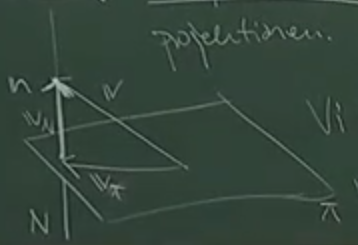
\includegraphics[scale=0.5]{imgs/img01.png}\\

$\bm{v}_{\pi}=\bm{v}-\bm{v}_{\bm{n}???}=\bm{v}-\frac{\bm{v}\cdot \bm{n}}{\bm{n} \cdot \bm{n}}\bm{n}$
Vi kan välja $\bm{n}=\begin{pmatrix}2&1&3\end{pmatrix}$.\\
Vi tar reda på $(\bm{e}_{x})_{pi}$, $(\bm{e}_{y})_{pi}$, $(\bm{e}_{z})_{pi}$
\begin{equation*}
    (\bm{e}_{x})_{pi}=
    \bm{e}_{x}-\frac{\bm{e}_{x}\cdot \bm{n}}{\bm{n}\cdot \bm{n}}=
    \begin{pmatrix}1\\0\\0\end{pmatrix}-\frac{\begin{pmatrix}1&0&0\end{pmatrix}\cdot \begin{pmatrix}2&1&3\end{pmatrix}}{\begin{pmatrix}2&1&3\end{pmatrix}\cdot \begin{pmatrix}2&1&3\end{pmatrix}}\begin{pmatrix}2\\1\\3\end{pmatrix}=
    \begin{pmatrix}1\\0\\0\end{pmatrix}-\frac{2}{14}\begin{pmatrix}2\\1\\3\end{pmatrix}=
    \frac{2}{14}\begin{pmatrix}10\\-2\\-6\end{pmatrix}
\end{equation*}

\begin{equation*}
    (\bm{e}_{y})_{pi}=
    \begin{pmatrix}0\\1\\0\end{pmatrix}-\frac{1}{14}\begin{pmatrix}2\\1\\3\end{pmatrix}=
    \frac{1}{14}\begin{pmatrix}-2\\-14\\-3\end{pmatrix}
\end{equation*}

\begin{equation*}
    (\bm{e}_{z})_{pi}=
    \begin{pmatrix}0\\0\\1\end{pmatrix}-\frac{3}{14}\begin{pmatrix}2\\1\\3\end{pmatrix}=
    \frac{1}{14}\begin{pmatrix}-6\\-3\\5\end{pmatrix}
\end{equation*}

Matrisen ges av $p=\begin{pmatrix}(\bm{e}_{x})_{pi} & (\bm{e}_{y})_{pi} & (\bm{e}_{z})_{pi}\end{pmatrix}=\frac{1}{14}\begin{pmatrix}
    10&-2&-6\\
    -2&-14&-3\\
    -6&-3&5
\end{pmatrix}$.\\

\underline{Relationen} Låt $R$ vara matrisen till rotationen.\\

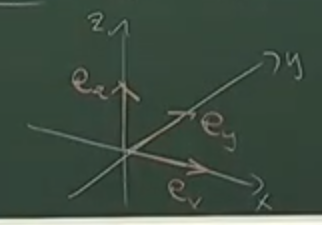
\includegraphics[scale=0.5]{imgs/img02.png}

\begin{equation*}
    R=\begin{pmatrix}
        1&0&0\\
        0&cos\frac{\pi}{3}&-sin\frac{\pi}{3}\\
        0&sin\frac{\pi}{3}&cos\frac{\pi}{3}
    \end{pmatrix}=
    \frac{1}{2}\begin{pmatrix}
        2&0&0\\
        0&cos\frac{\pi}{3}&-sin\frac{\pi}{3}\\
        0&\sqrt{3}&1
    \end{pmatrix}
\end{equation*}

Matrisen till $f$ ges av $RP$.\\
\begin{equation*}
    RP=\frac{1}{28}\begin{pmatrix}
        2&0&0\\
        0&1&-\sqrt{3}\\
        0&\sqrt{3}&1
    \end{pmatrix}\begin{pmatrix}
        10&-2&-6\\
        -2&-13&-3\\
        -6&-3&5
    \end{pmatrix}=
    \frac{1}{28}\begin{pmatrix}
        20&-4&-12\\
        -2+6\sqrt{3}&-13+3\sqrt{3}&-3-5\sqrt{3}\\
        -2\sqrt{3}-6&-13\sqrt{3}-3&-3\sqrt{3}+5
    \end{pmatrix}
\end{equation*}

\chapter{Area- och Volymförändringar (Avs 3.6)}
\begin{wrapfigure}{r}{0.5\textwidth}
    \vspace{-50pt}
    \centering
    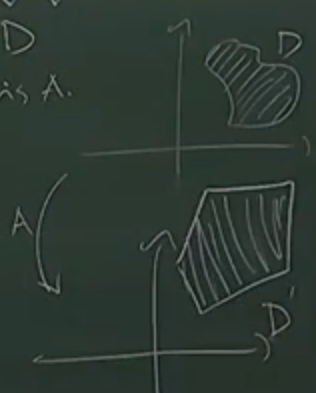
\includegraphics[scale=0.4]{imgs/img03.png}
    \vspace{-30pt}
\end{wrapfigure}
\paragraph{Sats 3.29} Antag att $D$ är ett godtyckligt område i planet.
Låt $D^{\prime}$ vara bilden av $D$ under den linjära avbildningen med matris $A$.\\
Då är $\frac{area(d^{\prime})}{area(d)}=|det(A)|$.
\\
\paragraph{Ex} Låt $D$ vara en rektangel i planet och $R$ vara en rotation.\\
Vad är arean av $R(D)$ eller då bilden av $D=D^{\prime}$?
\subparagraph{Lösning} Vi tycker att $arean(\prim{D})=arean(D)$.
Hur visar vi det?\\
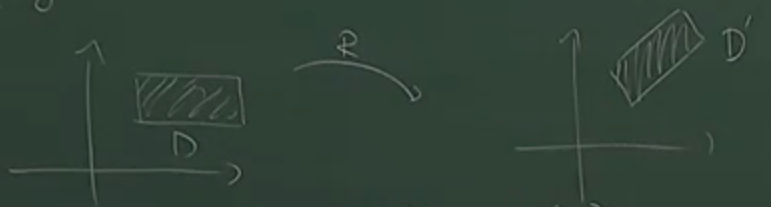
\includegraphics[scale=0.5]{imgs/img04.png}\\
Rotationer ges av $R=\begin{pmatrix}
    cos\beta&-sin\beta\\
    sin\beta&cos\beta
\end{pmatrix}$ och $det(R)=cos^{2}\beta+sin^{2}\beta=1$ så enligt sats 3.29 är $\frac{area(\prim{D})}{area(D)}=1$

\clearpage

\paragraph{Ex} Hur förändras arean av ett område under följande avbildningarna?
\begin{equation*}
    A=\begin{pmatrix}a&0\\0&1\end{pmatrix}\text{, }B=\begin{pmatrix}1&0\\0&b\end{pmatrix}\text{, }C=\begin{pmatrix}a&0\\0&b\end{pmatrix}
\end{equation*}

\subparagraph{Lösning} Engligt sats 3.29 så ges areaförändringen av determinanten:
\begin{equation*}
    det(A)=a\text{, }det(B)=b\text{, }det(C)=ab
\end{equation*}
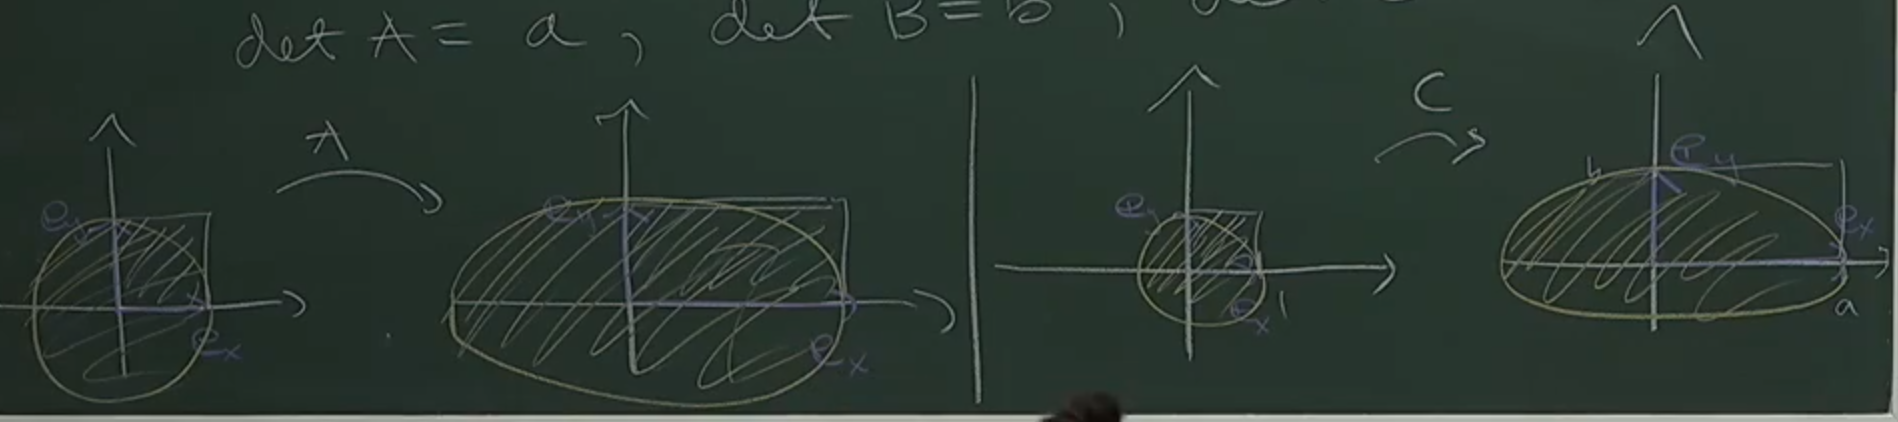
\includegraphics[scale=0.2]{imgs/img05.png}

\paragraph{Sats 3.31} Antag att $D$ är ett godtyckligt område i rummet och låt $\prim{D}$ vara bilden av $D$ under en linjär avbildning med matris $A$.
Då är
\begin{equation*}
    \frac{Volym(\prim{D})}{Volym(D)}=|det(A)|
\end{equation*}

\chapter{Affina avbildningar (Avs 3.7)}
Låt $V$ vara planet eller rummet och låt $\bm{b}$ vara en vektor i $V$.\\
Avbildningen $t_{\bm{b}}(\bm{v})=\bm{b}+\bm{v}$ kallas \underline{translationen med $\bm{b}$}.
Den är \underline{inte} linjär!\\
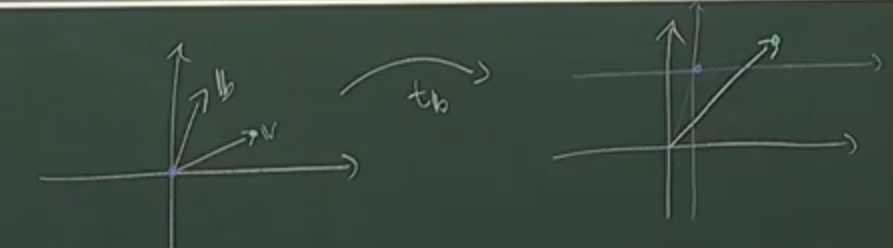
\includegraphics[scale=0.5]{imgs/img06.png}\\
Allting förflyttas med $\bm{b}$!\\
En funktion på formen $f(\bm{w})=A\bm{v}+\bm{b}$ sägs vara en \underline{affin avbildning}.
Affina avbildnigar liknar linjära avbildningar.
De avbildar linjer på linjer eller på punkter.
Sammansättningen av affina avbildningar är affin.\\
Varje linjär avbildning är också en affin avbildning (låt $\bm{b}=\bm{0}$).

\paragraph{Ex} $f(x)=kx$ är en affin och linjär avbildning. 
$g(x)=kx+m$ är inte linjär utan endast affin!

\chapter{Rummet  $\mathbb{R}^{n}$}
\section{Vektorer av allmän dimension (Avs 4.1)}
\paragraph{Definition} En \underline{vektor av dimension n}, n-vektor, $\bm{v}$är en n-tupel av reella tal och vi skriver
$\bm{v}=\begin{pmatrix}
    v_{1}\\
    v_{2}\\
    \vdots\\
    v_{n}
\end{pmatrix}$.
Mängden av alla n-vektorer är $\mathbb{R}^{n}$.\\
Vi låter 
\begin{itemize}
    \item[] 
        $\bm{u}+\bm{v}=
        \begin{pmatrix}
            u_{1}\\
            \vdots\\
            u_{n}
        \end{pmatrix}
            +
        \begin{pmatrix}
            v_{1}\\
            \vdots\\
            v_{n}
        \end{pmatrix}
        =
        \begin{pmatrix}
            u_{1}+v_{1}\\
            \vdots\\
            u_{n}+v_{n}
        \end{pmatrix}$
    \item[] $c\bm{v}=c\begin{pmatrix}
        v_{1}\\
        \vdots\\
        v_{n}
    \end{pmatrix}=\begin{pmatrix}
        cv_{1}\\
        \vdots\\
        cv_{n}
    \end{pmatrix}$
    \item[] $\bm{u}\cdot \bm{v}=\begin{pmatrix}u_{1}\\\vdots\\u_{n}\end{pmatrix}\cdot\begin{pmatrix}v_{1}\\\vdots\\v_{n}\end{pmatrix}= u_{1}v_{1}+u_{2}v_{2}+\ldots+u_{n}v_{n}$
    \item[] $||\bm{u}||=||\begin{pmatrix}u_{1}\\\vdots\\u_{n}\end{pmatrix}||=\sqrt{u_{1}^{2}+u_{2}^{2}+\ldots+u_{n}^{2}}$
\end{itemize}
\paragraph{Definition} 
\begin{itemize}
    \item[] Två vektorer $\bm{u}$ och $\bm{v}$ är \underline{parallella} om $\bm{u}=c\bm{v}$ för något $c\neq 0$.
    \item[] Två vektorer $\bm{u}$ och $\bm{v}$ är \underline{ortogonala} om $\bm{u}\cdot \bm{v}=0$.
    \item[] Vinkeln mellan $\bm{u}$ och $\bm{v}$ är det unika tal så att $cos\alpha=\frac{\bm{u}\cdot \bm{v}}{||\bm{u}||\cdot ||\bm{v}||}\text{ där } 0\leq \alpha \leq \pi$
\end{itemize}

\clearpage

\section{Räkneregler}
Vi får räkneregler såsom
\begin{itemize}
    \item[] $\bm{u}+\bm{v}=\bm{v}+\bm{u}$
    \item[] $(\bm{u}+\bm{v})+\bm{w}=\bm{u}+(\bm{v}+\bm{w})$
\end{itemize}
och så vidare... (Proposition 4.5)\\
\\
Pythagoras sats gäller: $\bm{u}$ och $\bm{v}$ är ortogonala $\Leftrightarrow ||\bm{u}+\bm{v}||^{2}=||\bm{u}||^{2}+||\bm{v}||^{2}$\\
\\
En vektor på formeln $a_{1}\bm{v}_{1}+a_{2}\bm{v}_{2}+\ldots+a_{m}\bm{v}_{m}$ är en \underline{linjärkombination av $\bm{v}_{1}+\bm{v}_{2}+\ldots+\bm{v}_{m}$}.
Standardbasen för $\mathbb{R}^{n}$ ges av $\bm{e}_{1}, \bm{e}_{2}, \ldots, \bm{e}_{n}$ där 
\begin{equation*}
    \bm{e}_{1}=\begin{pmatrix}
        1\\0\\\vdots\\0
    \end{pmatrix}\text{, }
    \bm{e}_{2}=\begin{pmatrix}
        0\\1\\\vdots\\0
    \end{pmatrix}\text{, }
    \ldots\text{, }
    \bm{e}_{n}=\begin{pmatrix}
        0\\0\\\vdots\\1
    \end{pmatrix}
\end{equation*}
\paragraph{Sats 4.11} Varje vektor i $\mathbb{R}^{n}$ går att skriva som en unik linjärkombination av $\bm{e}_{1},\bm{e}_{2},\ldots,\bm{e}_{m}$.
\begin{equation*}
    \begin{pmatrix}
        v_{1}\\
        v_{2}\\
        \vdots\\
        v_{m}
    \end{pmatrix}=
    v_{1}\bm{e}_{1}+v_{2}\bm{e}_{2}+\ldots+v_{n}\bm{e}_{n}
\end{equation*}